%!TEX root = ../../thesis.tex
\section{Some Sections}
\label{sec:sections}
This is the introduction~\cite{scipaper1, latex}\ldots
\vspace{1em}

\subsection{Fonts}

Test for fonts: Once Upon A Time,\ldots 01234577890
\vspace{1em}

serif (roman text): 
\textrm{Once Upon A Time,\ldots 01234577890} % or {\rmfamily Once Upon A Time,\ldots 01234577890}
\vspace{1em}

sans serif: 
\textsf{Once Upon A Time,\ldots 01234577890} % or {\sffamily Once Upon A Time,\ldots 01234577890}
\vspace{1em}

typewriter(monospace): 
\texttt{Once Upon A Time,\ldots 01234577890} % or {\ttfamily Once Upon A Time,\ldots 01234577890}
\vspace{1em}

medium: 
\textmd{Once Upon A Time,\ldots 01234577890} % or {\mdseries Once Upon A Time,\ldots 01234577890}
\vspace{1em}

bold:
\textbf{Once Upon A Time,\ldots 01234577890} % or {\bfseries Once Upon A Time,\ldots 01234577890}
\vspace{1em}

upright:
\textup{Once Upon A Time,\ldots 01234577890} % or {\upshape Once Upon A Time,\ldots 01234577890}
\vspace{1em}

italic:
\textit{Once Upon A Time,\ldots 01234577890} % or {\itshape Once Upon A Time,\ldots 01234577890}
\vspace{1em}

slanted:
\textsl{Once Upon A Time,\ldots 01234577890} % or {\slshape Once Upon A Time,\ldots 01234577890}
\vspace{1em}

small caps:
\textsc{Once Upon A Time,\ldots 01234577890} % or {\scshape Once Upon A Time,\ldots 01234577890}
\vspace{2em}

Test for maths of Euler-VM fonts:
$1234567890$, $1+1=2$,  $\int_0^1 dx = 1$, $\mathbold{abc\ldots z}$


\newpage
\subsection{Colors}
The template uses "xcolor" package with "dvipsnames" option to handle colors.

\begin{figure}[h!]
    \centering
    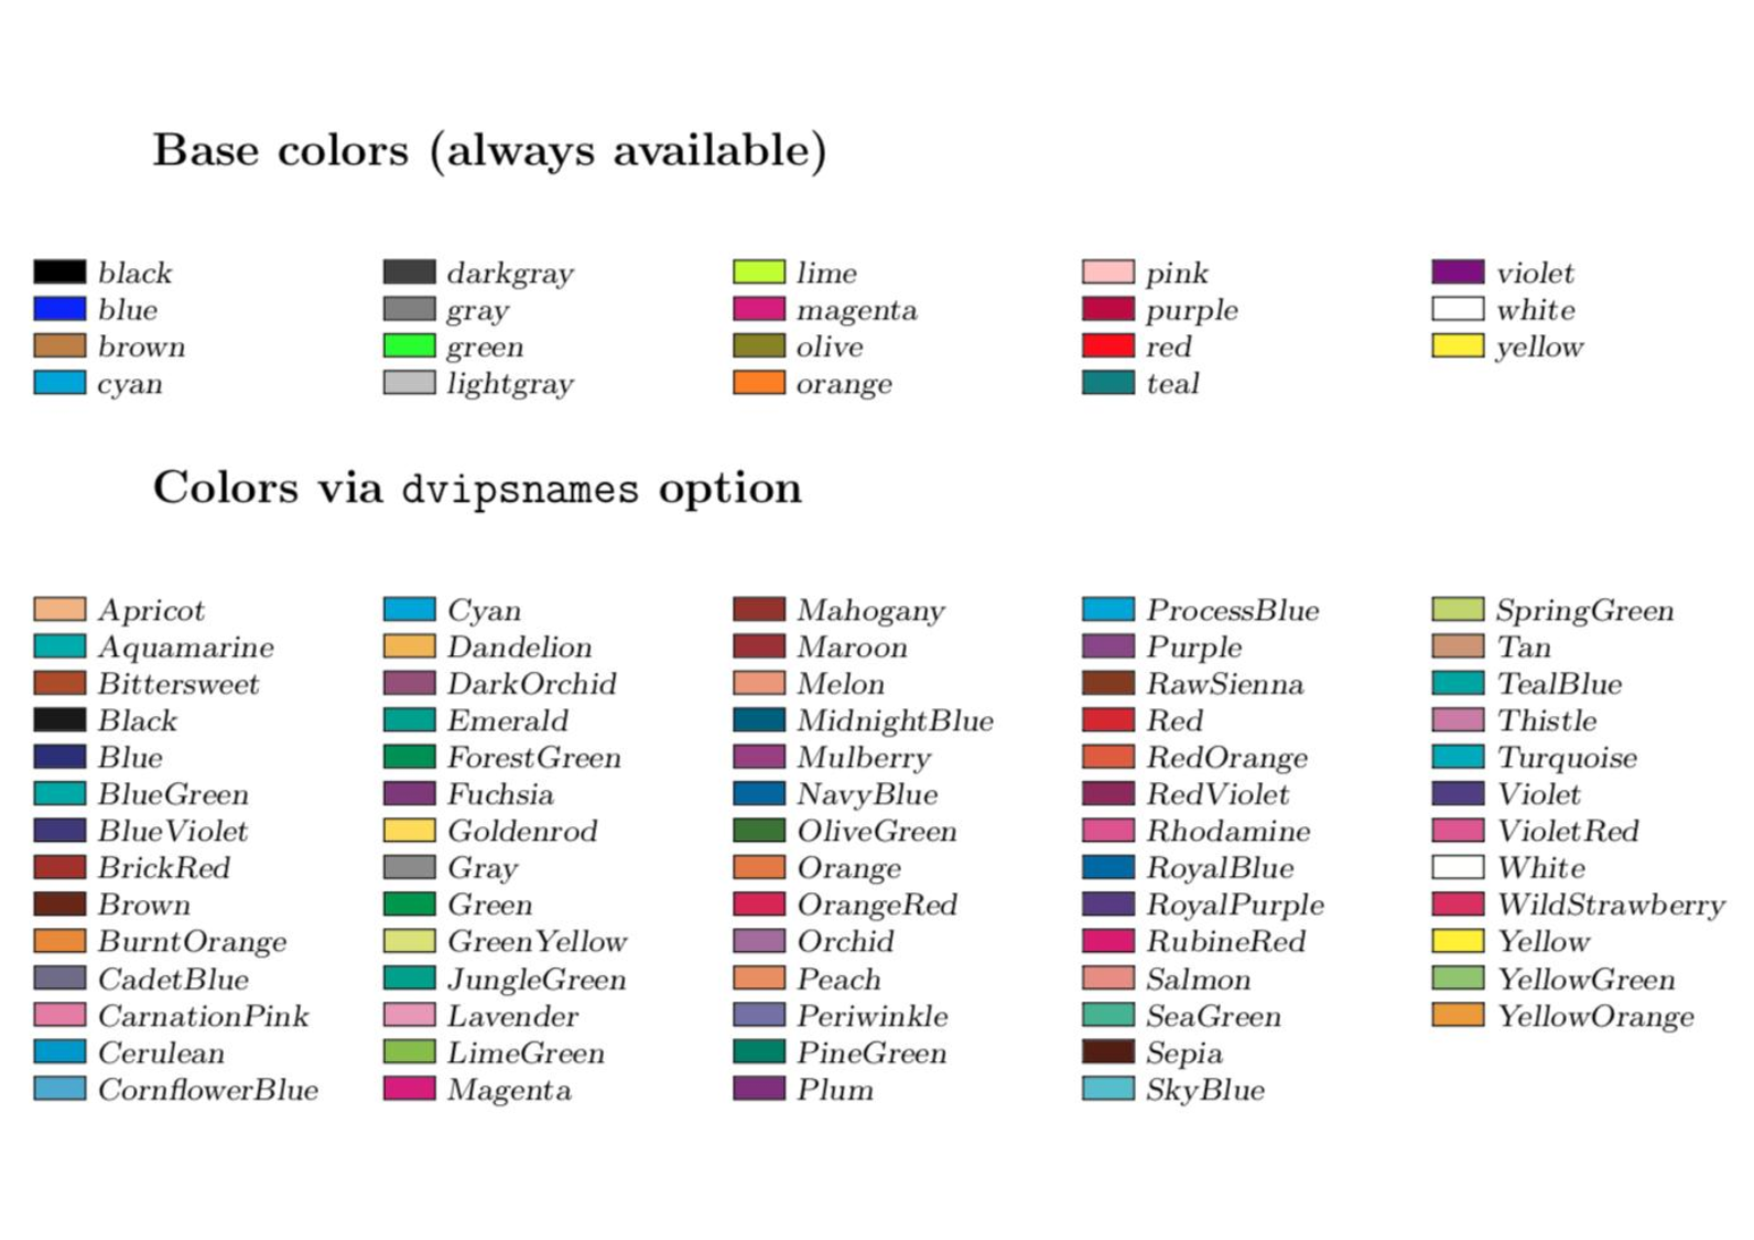
\includegraphics[width=0.9\textwidth]{chapter-1/sections/figs/colors.pdf}
    \caption{Colors from "xcolor" package with the "dvipsnames" option.}
\end{figure}

In addition to the basic colors and colors from "dvipsnames" option.
The template also defined a collection of colors based on the "Nord color theme
- an arctic, north-bluish color palette" from \url{https://www.nordtheme.com}.
For the detailed information for colors and style guides of the defined "nord" colors, please
check the Nord's web page
\url{https://www.nordtheme.com/docs/colors-and-palettes}. 

\noindent
Colors: Polar Night \\
\begin{tikzpicture}
\fill[nord0] (0,0) rectangle (1,1);
\fill[nord1] (1,0) rectangle (2,1);
\fill[nord2] (2,0) rectangle (3,1);
\fill[nord3] (3,0) rectangle (4,1);
\end{tikzpicture}

\noindent
Colors: Snow Storm \\
\begin{tikzpicture}
\fill[nord4] (0,0) rectangle (1,1);
\fill[nord5] (1,0) rectangle (2,1);
\fill[nord6] (2,0) rectangle (3,1);
\end{tikzpicture}

\noindent
Colors: Frost \\
\begin{tikzpicture}
\fill[nord7] (0,0) rectangle (1,1);
\fill[nord8] (1,0) rectangle (2,1);
\fill[nord9] (2,0) rectangle (3,1);
\fill[nord10] (3,0) rectangle (4,1);
\end{tikzpicture}

\noindent
Colors: Aurora \\
\begin{tikzpicture}
\fill[nord11] (0,0) rectangle (1,1);
\fill[nord12] (1,0) rectangle (2,1);
\fill[nord13] (2,0) rectangle (3,1);
\fill[nord14] (3,0) rectangle (4,1);
\fill[nord15] (4,0) rectangle (5,1);
\end{tikzpicture}

\newpage
\subsection{Test for a subsection} 
This is a test for subsection \ldots

\subsubsection{Test for a subsubsection}
This is a test for subsubsection \ldots 

\paragraph{Test for a paragraph} 
This is a test for paragraph \ldots

\subparagraph{Test for a subparagraph} 
This is a test for subparagraph \ldots 
